% ------------------------------------------------------------------------
% Configuração e Arquitetura do Template LaTeX
% Desenvolvido por: Aurora Drumond Costa Magalhães
% Ano: 2026
% ------------------------------------------------------------------------

\documentclass[
    12pt,
    openright,
    oneside,
    a4paper,
    english,
    brazil
    ]{abntex2}

% --- PACOTES GERAIS ---
\usepackage{lmodern}
\usepackage[T1]{fontenc}
\usepackage[utf8]{inputenc}
\usepackage{indentfirst}
\usepackage{graphicx}
\usepackage{float}
\usepackage[alf]{abntex2cite}

% --- CONFIGURAÇÃO DO AMBIENTE QUADRO ---
\newcommand{\quadroname}{Quadro}
\newcommand{\listofquadrosname}{Lista de quadros}

% Utilizando a sintaxe estrita do pacote 'float' (\newfloat{nome}{posicionamento}{extensão}[contador])
\floatstyle{plaintop} % Garante que a legenda fique acima do quadro
\newfloat{quadro}{htb}{loq}[chapter]
\floatname{quadro}{\quadroname}

% Cria a lista de quadros associada ao sumário
\newlistof{listofquadros}{loq}{\listofquadrosname}
\newlistentry{quadro}{loq}{0}

% Define a numeração contínua (evita Quadro 1.1, Quadro 1.2)
\counterwithout{quadro}{chapter}

% Configura a formatação de exibição da Lista de Quadros no PDF
\renewcommand{\cftquadroname}{\quadroname\space}
\renewcommand*{\cftquadroaftersnum}{\hfill--\hfill}

% --- IMPORTA SEUS ESTILOS PERSONALIZADOS ---
% Substitua pelos caminhos reais dos seus arquivos de estilo (.sty), caso possua.
\usepackage{styles/code-style} 
\usepackage{styles/mylib-style}

% --- DADOS DA CAPA ---
\titulo{Especificação e Projeto de Software: \\ Plataforma ``Preço Bão''}
\autor{Aurora Drumond Costa Magalhães \and Ana Clara de Souza \and Kayke Wellington}
\local{Timóteo - MG}
\data{2026}

\instituicao{%
  Centro Universitário Católica do Leste de Minas Gerais
  \par
  Campus Coronel Fabriciano}

% Mudamos de "Análise de auditoria" para o escopo real do trabalho
\tipotrabalho{Projeto de Engenharia de Software}

% O preâmbulo agora reflete a magnitude do seu projeto
\preambulo{Documentação completa de especificação, modelagem e arquitetura de software apresentada ao curso de Engenharia de Software do Centro Universitário Católica do Leste de Minas Gerais (Unileste).}

% --- INÍCIO DO DOCUMENTO ---
\begin{document}

% Elementos Pré-Textuais
\imprimircapa
\imprimirfolhaderosto

% Resumo (Pode ser movido para um arquivo chapters/00-resumos.tex se quiser)
\setlength{\absparsep}{18pt} % Ajusta o espaçamento dos parágrafos do resumo
\begin{resumo}
O presente trabalho documenta a especificação, a modelagem e a arquitetura do projeto ``Preço Bão'', uma plataforma computacional (aplicativo móvel e \textit{web}) voltada para a pesquisa, comparação e monitoramento de preços de medicamentos e produtos de farmácia. Motivada pela volatilidade dos valores no varejo farmacêutico e pela dificuldade de pesquisa física, a solução propõe um sistema alimentado por rotinas automatizadas e resilientes de extração de dados (\textit{web scraping}), construindo um catálogo centralizado. O escopo do documento abrange todas as fases de planejamento da Engenharia de Software. Inicialmente, são definidos o minimundo e o levantamento de requisitos funcionais e não funcionais, garantindo neutralidade algorítmica na busca, cálculo espacial de distância geolocalizada e rigoroso controle de privacidade adequado à LGPD. Em seguida, o projeto aprofunda-se na modelagem comportamental (Diagramas de Casos de Uso), no projeto de banco de dados (modelagem conceitual e lógica em PostgreSQL) e no \textit{design} estrutural e de interface. A arquitetura definida adota o padrão de \textit{monorepo}, provisionamento em contêineres, \textit{pipelines} de CI/CD, \textit{backend} assíncrono em Python (FastAPI) e \textit{frontend} multiplataforma em React Native. Como resultado, o trabalho entrega um planejamento arquitetural detalhado, robusto e escalável, preparando o sistema para a implementação codificada e garantindo uma ferramenta de alto impacto para o consumidor final.

\vspace{\onelineskip}
\noindent
\textbf{Palavras-chave:} Engenharia de Software. Especificação de Requisitos. \textit{Web Scraping}. Modelagem de Sistemas. Arquitetura de \textit{Software}.
\end{resumo}

% Abstract
\begin{resumo}[Abstract]
\begin{otherlanguage*}{english}
This paper documents the specification, modeling, and architecture of the ``Preço Bão'' project, a computational platform (mobile and web application) aimed at searching, comparing, and monitoring prices of medicines and pharmacy products. Driven by the price volatility in pharmaceutical retail and the challenge of physical searching, the solution proposes a system powered by automated and resilient data extraction routines (\textit{web scraping}) to build a centralized catalog. The document's scope covers all planning phases of Software Engineering. Initially, the domain and the elicitation of functional and non-functional requirements are defined, ensuring algorithmic neutrality in searches, spatial calculation of geolocated distance, and strict privacy controls compliant with data protection laws. Subsequently, the project delves into behavioral modeling (Use Case Diagrams), database design (conceptual and logical modeling in PostgreSQL), and structural and interface design. The defined architecture adopts a monorepo pattern, container provisioning, CI/CD pipelines, an asynchronous Python backend (FastAPI), and a cross-platform React Native frontend. As a result, the work delivers a detailed, robust, and scalable architectural plan, preparing the system for coding implementation and ensuring a high-impact tool for the end consumer.

\vspace{\onelineskip}
\noindent
\textbf{Keywords:} Software Engineering. Requirements Specification. Web Scraping. Systems Modeling. Software Architecture.
\end{otherlanguage*}
\end{resumo}

% Listas
% \pdfbookmark[0]{\listfigurename}{lof}
% \listoffigures*
% \cleardoublepage

% \pdfbookmark[0]{\lstlistlistingname}{lol}
% \lstlistoflistings
% \cleardoublepage

\pdfbookmark[0]{Lista de quadros}{loq}
\listofquadros*
\cleardoublepage

\pdfbookmark[0]{\contentsname}{toc}
\tableofcontents
\cleardoublepage

% --------------------------------------------------------
% ELEMENTOS TEXTUAIS
% --------------------------------------------------------
\textual

% Aqui acontece a mágica: você chama os arquivos externos

%\include{capitulos/01-introducao}
\chapter{Desenvolvimento}

Este capítulo tem como objetivo detalhar a concepção e a estruturação do projeto ``Preço Bão''. Nas seções a seguir, serão apresentados os elementos fundamentais para a compreensão do escopo do sistema, iniciando pela delimitação do minimundo, que descreve o domínio do problema, os fluxos operacionais e os principais requisitos que guiarão a modelagem do banco de dados e a arquitetura do software.

\section{Minimundo}

O projeto consiste em uma plataforma de serviço, acessível via aplicativo móvel e site, voltada para ajudar o consumidor final a pesquisar, comparar e monitorar os preços de medicamentos e produtos de farmácia.

O sistema é alimentado por uma rotina automatizada de extração de dados (\textit{web scraping}\footnote{Técnica computacional automatizada em que um \textit{script} ou algoritmo navega por páginas da web com o objetivo de raspar, coletar e estruturar em um banco de dados as informações públicas que originalmente são exibidas de forma não estruturada em código HTML.}) que varre os sites de diversas farmácias da região. Durante esse processo, o sistema coleta, processa e armazena informações vitais, como a disponibilidade dos produtos, os laboratórios fabricantes e os valores cobrados, construindo um grande catálogo centralizado de remédios.

Através da interface do aplicativo, o usuário final pode pesquisar pelos medicamentos de uso contínuo ou produtos que precisa comprar. O sistema então apresenta os produtos em cartões de exibição, listando as informações do laboratório e comparando os melhores preços encontrados no mercado. Para auxiliar ainda mais na decisão de compra, o aplicativo recebe as coordenadas geográficas do usuário e calcula matematicamente a distância entre ele e cada farmácia que possui o produto em estoque.

Por fim, o sistema permite que o usuário salve e acompanhe ativamente a mudança de preços dos remédios ao longo do tempo, garantindo que ele sempre saiba o momento e o local mais adequados para realizar sua compra.

\section{Especificação de Requisitos}

Nesta seção, os requisitos do sistema ``Preço Bão'' são detalhados e classificados. Os Requisitos Funcionais (RF) descrevem as ações e comportamentos que o sistema deve executar para atender às necessidades do usuário, enquanto os Requisitos Não Funcionais (RNF) especificam os critérios de qualidade, restrições tecnológicas e de desempenho que o sistema deve respeitar.

\begin{quadro}[H]
    \centering
    \caption{Especificação dos Requisitos Funcionais}
    \label{qua:requisitos_funcionais}
    \begin{tabularx}{\textwidth}{|c|X|}
        \hline
        \textbf{ID} & \textbf{Descrição do Requisito} \\
        \hline
        RF01 & \textbf{Extração Resiliente de Dados:} O sistema deve possuir uma rotina automatizada de \textit{web scraping} para coletar dados de farmácias. Em caso de falha na extração, o sistema deve registrar o erro em \textit{log} e continuar a varredura nas demais fontes. \\
        \hline
        RF02 & \textbf{Processamento e Catálogo:} O sistema deve armazenar as informações vitais extraídas e enriquecê-las contra a base da CMED/ANVISA. A disponibilidade em estoque deve ser exibida com um aviso claro de que é uma ``estimativa sujeita a confirmação no local''. \\
        \hline
        RF03 & \textbf{Gestão de Usuários:} O aplicativo deve permitir o cadastro de novos usuários, autenticação (\textit{login}) e recuperação de senha, criando um perfil individual. \\
        \hline
        RF04 & \textbf{Pesquisa e Neutralidade Algorítmica:} O consumidor deve poder pesquisar por medicamentos. O algoritmo de ordenação deve garantir a neutralidade, priorizando estritamente o menor preço ou a menor distância. \\
        \hline
        RF05 & \textbf{Exibição em Cartões:} O sistema deve exibir os resultados em cartões padronizados, listando informações do laboratório e comparando os melhores preços. \\
        \hline
        RF06 & \textbf{Cálculo de Distância Geográfica:} Mediante autorização prévia, o aplicativo deve receber as coordenadas geográficas do usuário e calcular a distância até os estabelecimentos, ordenando por proximidade. \\
        \hline
        RF07 & \textbf{Salvamento de Produtos:} O sistema deve permitir que um usuário autenticado favorite medicamentos de uso contínuo em sua conta. \\
        \hline
        RF08 & \textbf{Monitoramento de Preços:} O sistema deve gerar e exibir um gráfico ou histórico rastreando a flutuação de preços dos remédios salvos ao longo das últimas semanas. \\
        \hline
    \end{tabularx}
    \fonte{Elaborado pelos autores (2026).}
\end{quadro}

\vspace{0.5cm}

\begin{quadro}[H]
    \centering
    \caption{Requisitos Não Funcionais: Arquitetura e Performance}
    \label{qua:rnf_arquitetura}
    \begin{tabularx}{\textwidth}{|c|X|}
        \hline
        \textbf{ID} & \textbf{Descrição do Requisito} \\
        \hline
        RNF01 & \textbf{Performance da API:} O \textit{backend} (Python/FastAPI) deve ser assíncrono e responder a requisições de pesquisa em um tempo máximo de 500 milissegundos no percentil 95. \\
        \hline
        RNF02 & \textbf{Arquitetura do Frontend:} O aplicativo móvel deve ser desenvolvido com React Native e Expo utilizando TypeScript, garantindo \textit{builds} funcionais para Android e iOS. \\
        \hline
        RNF03 & \textbf{Persistência e Retenção:} Os dados devem ser armazenados em um PostgreSQL. O sistema deve implementar uma política de limpeza (\textit{data purging}), excluindo históricos com mais de 12 meses. \\
        \hline
    \end{tabularx}
    \fonte{Elaborado pelos autores (2026).}
\end{quadro}

\vspace{0.5cm}

\begin{quadro}[H]
    \centering
    \caption{Requisitos Não Funcionais: Segurança e Conformidade}
    \label{qua:rnf_seguranca}
    \begin{tabularx}{\textwidth}{|c|X|}
        \hline
        \textbf{ID} & \textbf{Descrição do Requisito} \\
        \hline
        RNF04 & \textbf{Segurança e Criptografia:} Todas as senhas devem ser armazenadas utilizando \textit{hashing} fortes (ex: bcrypt). A comunicação deve ocorrer obrigatoriamente sob protocolo HTTPS/TLS. \\
        \hline
        RNF05 & \textbf{Privacidade (LGPD):} O sistema não deve armazenar o histórico contínuo de localização do usuário. As coordenadas devem ser processadas em memória e descartadas em seguida. \\
        \hline
    \end{tabularx}
    \fonte{Elaborado pelos autores (2026).}
\end{quadro}

\vspace{0.5cm}

\begin{quadro}[H]
    \centering
    \caption{Requisitos Não Funcionais: Engenharia e Qualidade de Código}
    \label{qua:rnf_engenharia}
    \begin{tabularx}{\textwidth}{|c|X|}
        \hline
        \textbf{ID} & \textbf{Descrição do Requisito} \\
        \hline
        RNF06 & \textbf{Estrutura e Validação:} O sistema deve utilizar ORM e Pydantic no \textit{backend} para validação. O TypeScript no \textit{frontend} deve usar modo estrito (\code{strict: true}). \\
        \hline
        RNF07 & \textbf{Organização em Monorepo:} O projeto deve adotar a estrutura de monorepo, isolando as dependências do \textit{frontend} e do \textit{backend}. \\
        \hline
        RNF08 & \textbf{Orquestração Local:} O ambiente de desenvolvimento deve ser provisionado via \file{docker-compose.yml}. \\
        \hline
        RNF09 & \textbf{Automação de Comandos:} O repositório deve conter um \file{Makefile} na raiz para abstrair comandos complexos (ex: \code{make up}). \\
        \hline
        RNF10 & \textbf{CI/CD e Qualidade:} Fluxos do GitHub Actions devem bloquear \textit{Pull Requests} que falhem nos testes ou na análise estática (ESLint/Ruff). \\
        \hline
        RNF11 & \textbf{Padronização de Estilo:} O repositório deve impor formatação via \file{.editorconfig} e possuir um \file{.gitignore} rigoroso para blindar chaves secretas. \\
        \hline
    \end{tabularx}
    \fonte{Elaborado pelos autores (2026).}
\end{quadro}

\section{Modelagem do Sistema}

Com os requisitos funcionais e não funcionais devidamente especificados, a etapa seguinte no desenvolvimento do projeto consiste na abstração e representação visual dessas regras de negócio. Para isso, utiliza-se a Linguagem de Modelagem Unificada (UML), que atua como uma ponte padronizada entre a especificação em linguagem natural e a implementação técnica.

\subsection{Diagrama de Casos de Uso}

O diagrama de casos de uso tem como objetivo principal mapear as interações entre os atores (usuários finais e sistemas externos) e as funcionalidades delimitadas pela fronteira do sistema. Segundo Booch, Rumbaugh e Jacobson (2005), essa modelagem comportamental é essencial para documentar o comportamento do \textit{software} a partir da perspectiva de quem o utiliza, garantindo a validação do escopo definido nos requisitos funcionais.

A Figura \ref{fig:diagrama_casos_de_uso} ilustra o diagrama projetado para a plataforma ``Preço Bão''. Destacam-se na modelagem as relações de dependência estereotipadas. O relacionamento de inclusão (\textit{$\ll$include$\gg$}) demonstra que ações como favoritar produtos, monitorar histórico ou gerenciar o perfil exigem, obrigatoriamente, a prévia autenticação do usuário. Por outro lado, o relacionamento de extensão (\textit{$\ll$extend$\gg$}) indica que o cálculo de distância geográfica atua como um fluxo alternativo e opcional à pesquisa base, ocorrendo apenas mediante a concessão de permissões de localização do dispositivo.

Adicionalmente, a arquitetura contempla a comunicação de retaguarda do sistema com a base de dados abertos da Câmara de Regulação do Mercado de Medicamentos (CMED/ANVISA). Esta integração configura um caso de uso sistêmico (\textit{background job}) responsável pela ingestão, cruzamento e validação farmacológica dos códigos de barras extraídos pelo robô de \textit{scraping}, mitigando integralmente a dependência de APIs de terceiros.

\begin{figure}[htb]
    \centering
    \caption{Diagrama de Casos de Uso da Plataforma Preço Bão}
    \label{fig:diagrama_casos_de_uso}
    % Lembre-se de ajustar a extensão do arquivo se for .png ou .jpg
    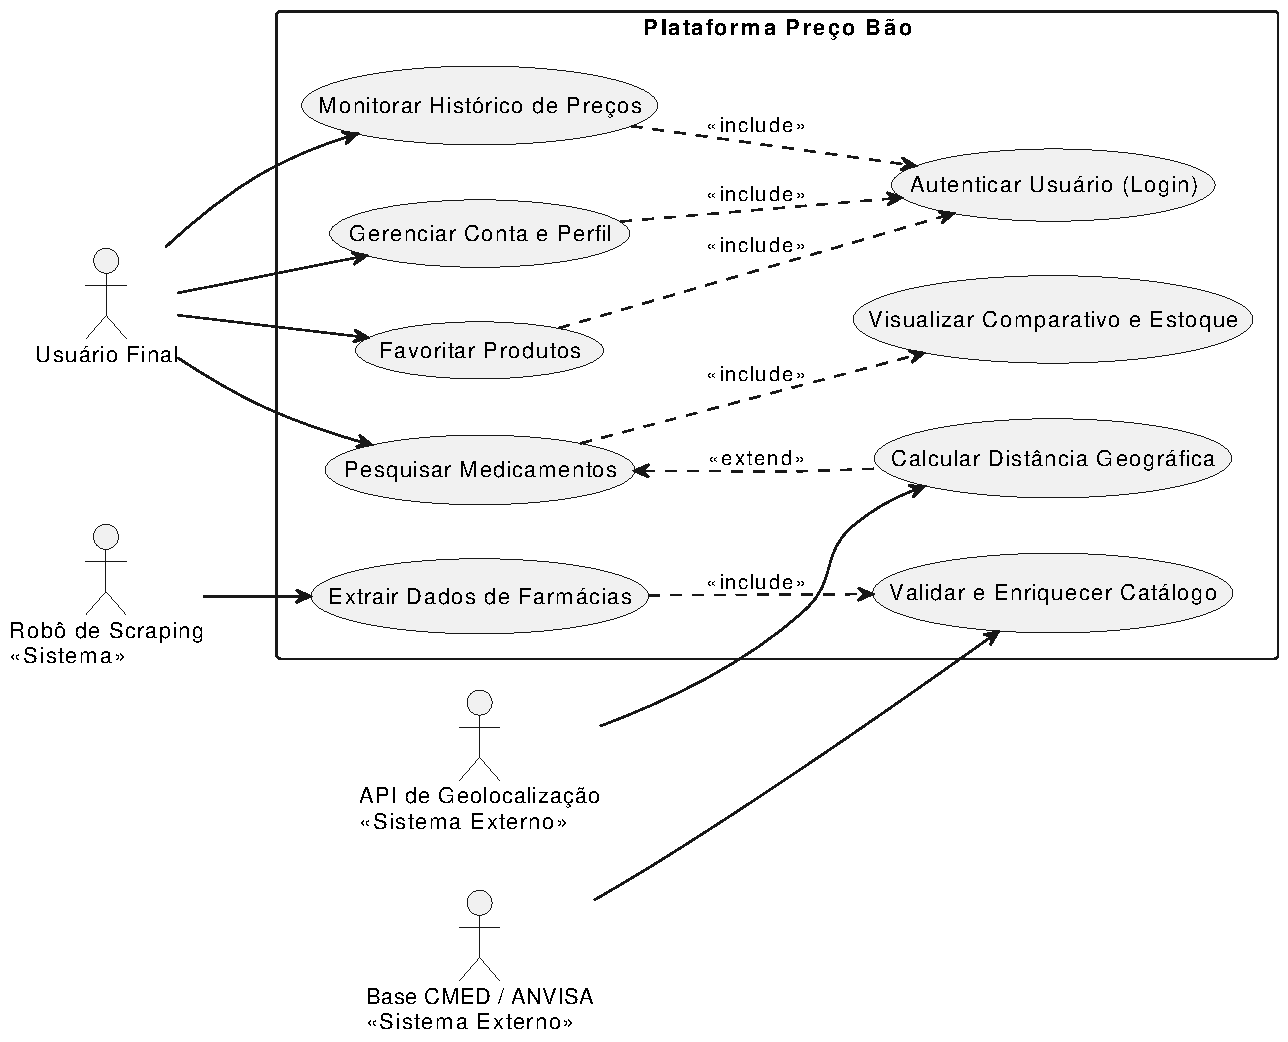
\includegraphics[width=\textwidth]{figures/diagrama-caso-de-uso.pdf} 
    \fonte{Elaborado pelos autores (2026).}
\end{figure}

\subsection{Diagrama de Classes}

Enquanto o diagrama de casos de uso foca no comportamento externo e nas interações dos atores com o sistema, o diagrama de classes detalha a estrutura estática interna da aplicação. Segundo Larman (2007), este artefato é fundamental no projeto orientado a objetos, pois ilustra as entidades lógicas, seus atributos, operações e os relacionamentos que sustentam a arquitetura do \textit{software}. Para a plataforma ``Preço Bão'', a modelagem estrutural foi projetada refletindo a separação de responsabilidades do sistema, delineando o percurso da informação desde a sua coleta até a persistência no banco de dados. 

Para facilitar a visualização e a compreensão arquitetural, a modelagem foi dividida em três agrupamentos lógicos principais, detalhados a seguir.

\subsubsection{Motor de \textit{Scraping} (ETL)}

Este primeiro grupo encapsula a rotina automatizada de extração de dados. Para garantir escalabilidade e facilitar a futura inclusão de novas redes de farmácias, adotou-se o uso de abstração no padrão de projeto. A Figura \ref{fig:diagrama_scraping} ilustra a superclasse abstrata \texttt{BaseScraper}, que define o contrato padrão e os métodos obrigatórios (como \texttt{extrair\_todos\_produtos()}). Classes concretas, a exemplo de \texttt{IndianaScraper}, herdam essa estrutura e implementam as particularidades (HTML ou JSON) de cada loja, promovendo o reaproveitamento de código e o polimorfismo.

\begin{figure}[htb]
    \centering
    \caption{Diagrama de Classes: Motor de Scraping (ETL)}
    \label{fig:diagrama_scraping}
    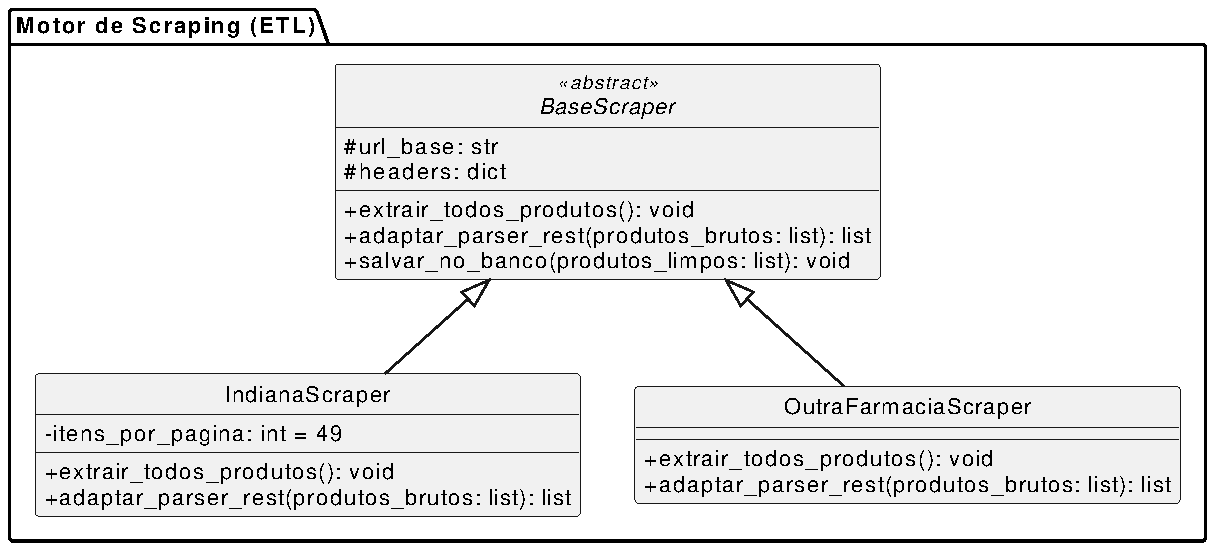
\includegraphics[width=0.8\textwidth]{figures/diagrama-scraping.pdf} 
    \fonte{Elaborado pelos autores (2026).}
\end{figure}

A estrutura interna deste módulo, conforme ilustrada, é composta pelas seguintes classes principais:

\begin{itemize}
    \item \textbf{\texttt{BaseScraper}:} Atua como a superclasse abstrata do módulo. Ela define os atributos protegidos essenciais para a configuração das requisições HTTP (como \texttt{url\_base} e \texttt{headers}) e estabelece um contrato arquitetural rigoroso. Para isso, utiliza métodos abstratos que devem, obrigatoriamente, ser sobrescritos pelas subclasses, a exemplo de \texttt{extrair\_todos\_produtos()} e \texttt{adaptar\_parser\_rest()}. Além de ditar as regras de extração, a superclasse encapsula o reaproveitamento de código no método concreto \texttt{salvar\_no\_banco()}, assegurando que todos os dados limpos sejam inseridos de forma padronizada no banco de dados, independentemente de sua origem.

    \item \textbf{\texttt{IndianaScraper}:} Consiste na implementação concreta desenvolvida para interagir com o catálogo da rede Farmácia Indiana. Herdando as propriedades da classe base, ela materializa as regras de negócio específicas desta loja. A classe define o atributo privado \texttt{itens\_por\_pagina = 49} para mapear o limite da API da farmácia e implementa a lógica exata de varredura e de tratamento (conversão do JSON bruto da API VTEX para os DTOs do sistema) em seus respectivos métodos.

    \item \textbf{\texttt{OutraFarmaciaScraper}:} Trata-se de uma classe de representação que evidencia a escalabilidade e a extensibilidade da arquitetura projetada. Sua inclusão no diagrama demonstra o atendimento ao Princípio Aberto/Fechado (\textit{Open/Closed Principle} do SOLID): a plataforma está aberta para expansão (adição de novos robôs para outras redes de farmácias através de herança) e fechada para modificação (a lógica central do motor e a persistência não precisam ser alteradas para suportar uma nova fonte de dados).
\end{itemize}

\subsubsection{\textit{Schemas} da API (Pydantic)}

O segundo agrupamento representa a camada de validação e transferência de dados (\textit{Data Transfer Objects} - DTOs) utilizada pelo \textit{framework} FastAPI. Através da herança da classe \texttt{BaseModel}, conforme demonstrado na Figura \ref{fig:diagrama_schemas}, são definidos os formatos exatos que transitam na rede. Essa divisão permite que uma mesma entidade lógica possua representações distintas para contextos diferentes, isolando dados sensíveis nas requisições (como \texttt{UsuarioCreate}, que exige senha clara) e omitindo-os nas respostas públicas (como \texttt{UsuarioOut}).

\begin{figure}[H]
    \centering
    \caption{Diagrama de Classes: Schemas da API (Pydantic)}
    \label{fig:diagrama_schemas}
    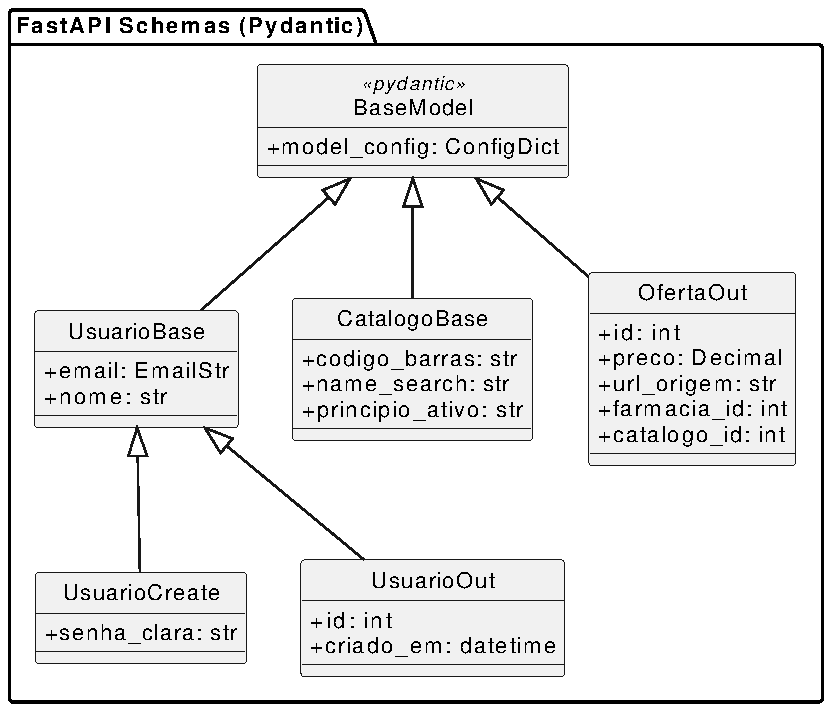
\includegraphics[width=0.7\textwidth]{figures/diagrama-schemas.pdf} 
    \fonte{Elaborado pelos autores (2026).}
\end{figure}

A modelagem desta camada de transferência de dados é estruturada em torno das seguintes classes e padrões de herança:

\begin{itemize}
    \item \textbf{\texttt{BaseModel}:} Classe fundamental proveniente da biblioteca Pydantic. Ela fornece o motor de validação estrita, tipagem e serialização/desserialização dos dados em formato JSON. O atributo \texttt{model\_config} (do tipo \texttt{ConfigDict}) permite estabelecer diretrizes globais para os \textit{schemas}, garantindo a segurança e a integridade das requisições recebidas pela API.

    \item \textbf{Família de \textit{Schemas} de Usuário (\texttt{UsuarioBase}, \texttt{UsuarioCreate}, \texttt{UsuarioOut}):} Demonstra a aplicação da segregação de responsabilidades nos DTOs. A classe \texttt{UsuarioBase} agrupa atributos universais (como \texttt{email} e \texttt{nome}). A partir dela, deriva-se a classe \texttt{UsuarioCreate}, utilizada exclusivamente nos métodos de cadastro (\textit{POST}) e que inclui o dado sensível \texttt{senha\_clara}. Em contrapartida, a classe \texttt{UsuarioOut} formata a resposta pública da API, incorporando atributos gerados pelo banco de dados (\texttt{id} e \texttt{criado\_em}), omitindo terminantemente qualquer informação de autenticação.

    \item \textbf{Família de \textit{Schemas} de Catálogo e Ofertas (\texttt{CatalogoBase}, \texttt{OfertaOut}):} Em alinhamento com a separação estrutural do banco de dados, os \textit{schemas} separam os dados universais do produto de suas ocorrências locais no varejo. Os DTOs de catálogo trafegam os dados farmacológicos (como \texttt{codigo\_barras} e \texttt{principio\_ativo}), enquanto a herança de ofertas é utilizada para devolver esses dados consolidados ao \textit{frontend}, acrescentando as propriedades voláteis (como o \texttt{preco}) e metadados de rastreabilidade (como a \texttt{url\_origem}).
\end{itemize}

\subsubsection{Mapeamento Objeto-Relacional (SQLAlchemy ORM)}

Por fim, o terceiro grupo consolida as entidades físicas que compõem o esquema relacional do banco de dados PostgreSQL. A Figura \ref{fig:diagrama_orm} apresenta o mapeamento central das classes de domínio. A modelagem desta camada sofreu uma importante refatoração estrutural (abandono do monólito de produto) para garantir escalabilidade, estabelecendo uma separação estrita entre o catálogo farmacológico imutável e as ofertas de mercado voláteis. O diagrama mapeia os atributos tipados, as chaves primárias e, sobretudo, os relacionamentos por meio de chaves estrangeiras. 

\begin{figure}[htb]
    \centering
    \caption{Diagrama de Classes: Banco de Dados (SQLAlchemy ORM)}
    \label{fig:diagrama_orm}
    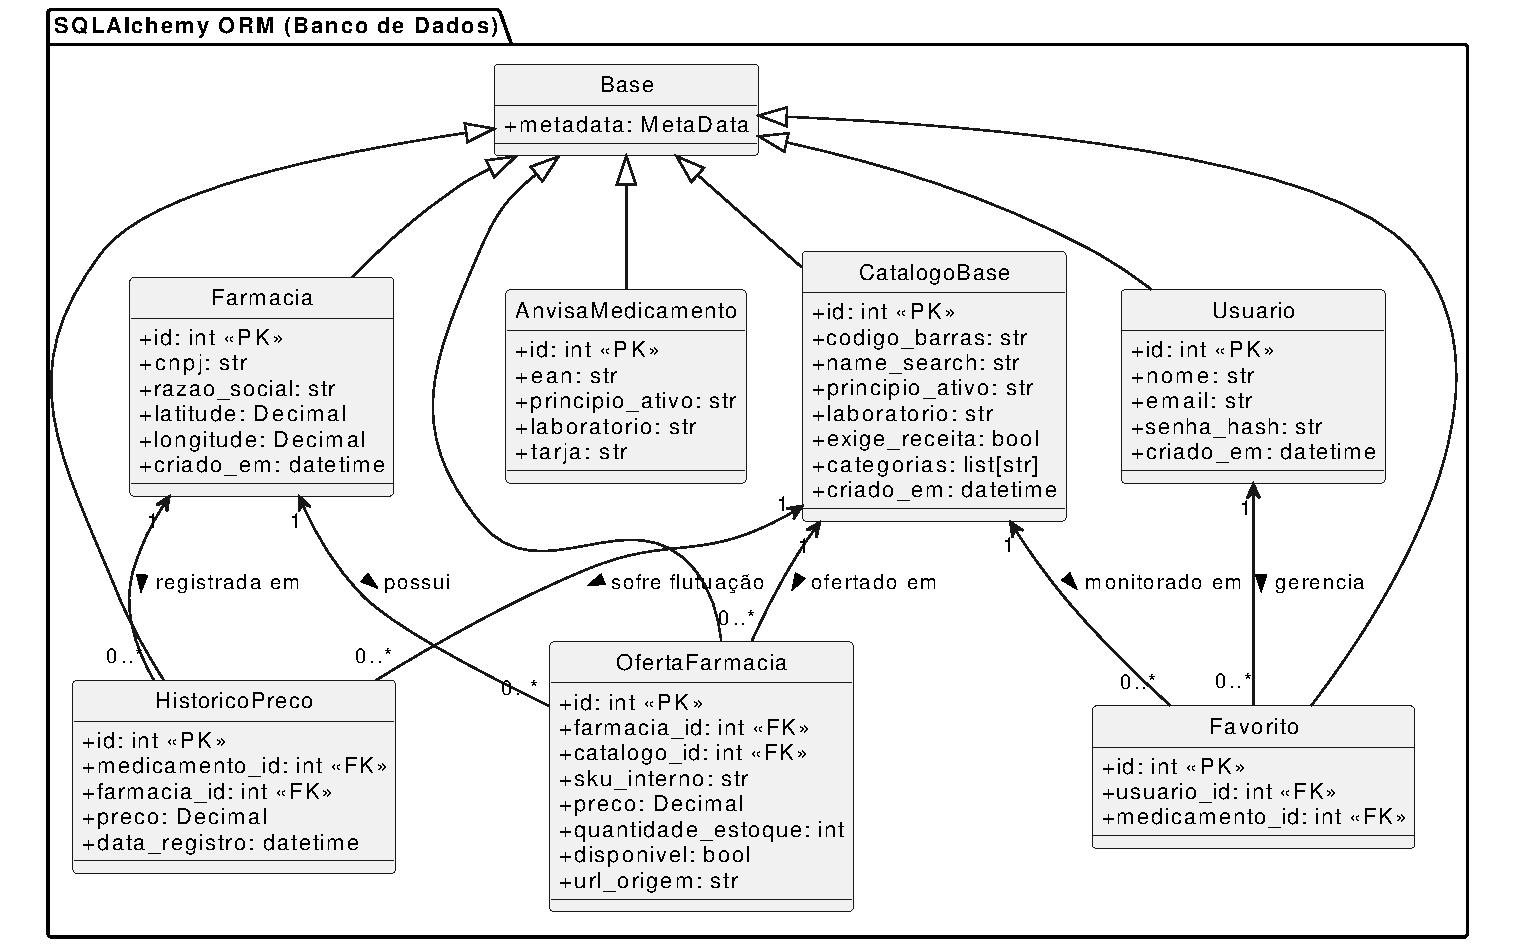
\includegraphics[width=\textwidth]{figures/diagrama-orm.pdf} 
    \fonte{Elaborado pelos autores (2026).}
\end{figure}

O detalhamento estrutural deste agrupamento revela as entidades centrais do domínio e suas respectivas responsabilidades atualizadas:

\begin{itemize}
    \item \textbf{\texttt{Base}:} Atua como o alicerce do mapeamento objeto-relacional. Todas as demais tabelas herdam desta classe declarativa, que injeta centralmente as convenções de nomenclatura e gerencia os metadados (\texttt{MetaData}) essenciais para a estabilidade das migrações automáticas de esquema.
    
    \item \textbf{\texttt{CatalogoBase}:} Representa o catálogo unificado da plataforma. Armazena exclusivamente os dados farmacológicos e invariáveis do produto (como \texttt{codigo\_barras}, \texttt{principio\_ativo}, \texttt{categorias} organizacionais em \textit{array} e a coluna \texttt{name\_search} indexada para otimização de buscas textuais). Atua como a identidade de referência para todas as lojas.

    \item \textbf{\texttt{Farmacia} e \texttt{OfertaFarmacia}:} A entidade \texttt{Farmacia} armazena os dados físicos e corporativos, com destaque para os atributos \texttt{latitude} e \texttt{longitude}, viabilizando o requisito de cálculo de distanciamento espacial. A entidade \texttt{OfertaFarmacia} atua como a resolução associativa do estoque, gerenciando os dados voláteis de varejo (\texttt{preco}, \texttt{quantidade\_estoque}, disponibilidade e o identificador \texttt{sku\_interno} da loja), estabelecendo relacionamento de muitos-para-muitos entre as \texttt{Farmacias} e o \texttt{CatalogoBase}.

    \item \textbf{\texttt{AnvisaMedicamento}:} Tabela de \textit{lookup} alimentada via \textit{scripts} de ingestão com os dados abertos da CMED/ANVISA. É utilizada pela infraestrutura para o enriquecimento e a sanitização interna dos dados coletados através do EAN, suprimindo o uso de APIs pagas ou instáveis de terceiros para a validação do catálogo.

    \item \textbf{\texttt{Usuario} e \texttt{Favorito}:} O \texttt{Usuario} encapsula os dados cadastrais e o vetor de autenticação (\texttt{senha\_hash}) do consumidor final. A entidade \texttt{Favorito} atua como uma ponte relacional, conectando a chave do usuário (\texttt{usuario\_id}) ao \texttt{CatalogoBase} (\texttt{medicamento\_id}), permitindo que o consumidor monitore um item independentemente de qual farmácia possua o melhor preço atual.
    
    \item \textbf{\texttt{HistoricoPreco}:} Classe dedicada a garantir a rastreabilidade financeira e auditoria de variações. Ela registra temporalmente os \textit{snapshots} de preço apontando obrigatoriamente tanto para o medicamento (\texttt{medicamento\_id}) quanto para o estabelecimento exato que praticou aquele valor (\texttt{farmacia\_id}). Essa estrutura composta garante a integridade lógica exigida para a plotagem dos gráficos de flutuação exibidos ao usuário.
\end{itemize}


\section{Protótipo de Interface e Navegação}

Após a consolidação dos requisitos e a estruturação da arquitetura de dados, a etapa seguinte no desenvolvimento centrou-se na tangibilização da experiência do usuário (UX) e no design de interface (UI). Para alinhar as expectativas visuais e validar o fluxo de interação antes da codificação, foi desenvolvido um protótipo de baixa a média fidelidade utilizando a ferramenta Figma. 

O objetivo do protótipo é mapear a jornada do consumidor dentro do aplicativo, garantindo que as funcionalidades descritas nos Requisitos Funcionais, como pesquisa e geolocalização, sejam facilmente acessíveis. A Figura \ref{fig:prototipo_telas} apresenta as principais telas que compõem a navegação central da plataforma ``Preço Bão''.

\begin{figure}[htb]
    \centering
    \caption{Protótipo de Telas da Plataforma Preço Bão}
    \label{fig:prototipo_telas}
    % Lembre-se de ajustar a extensão do arquivo se for .png ou .jpg
    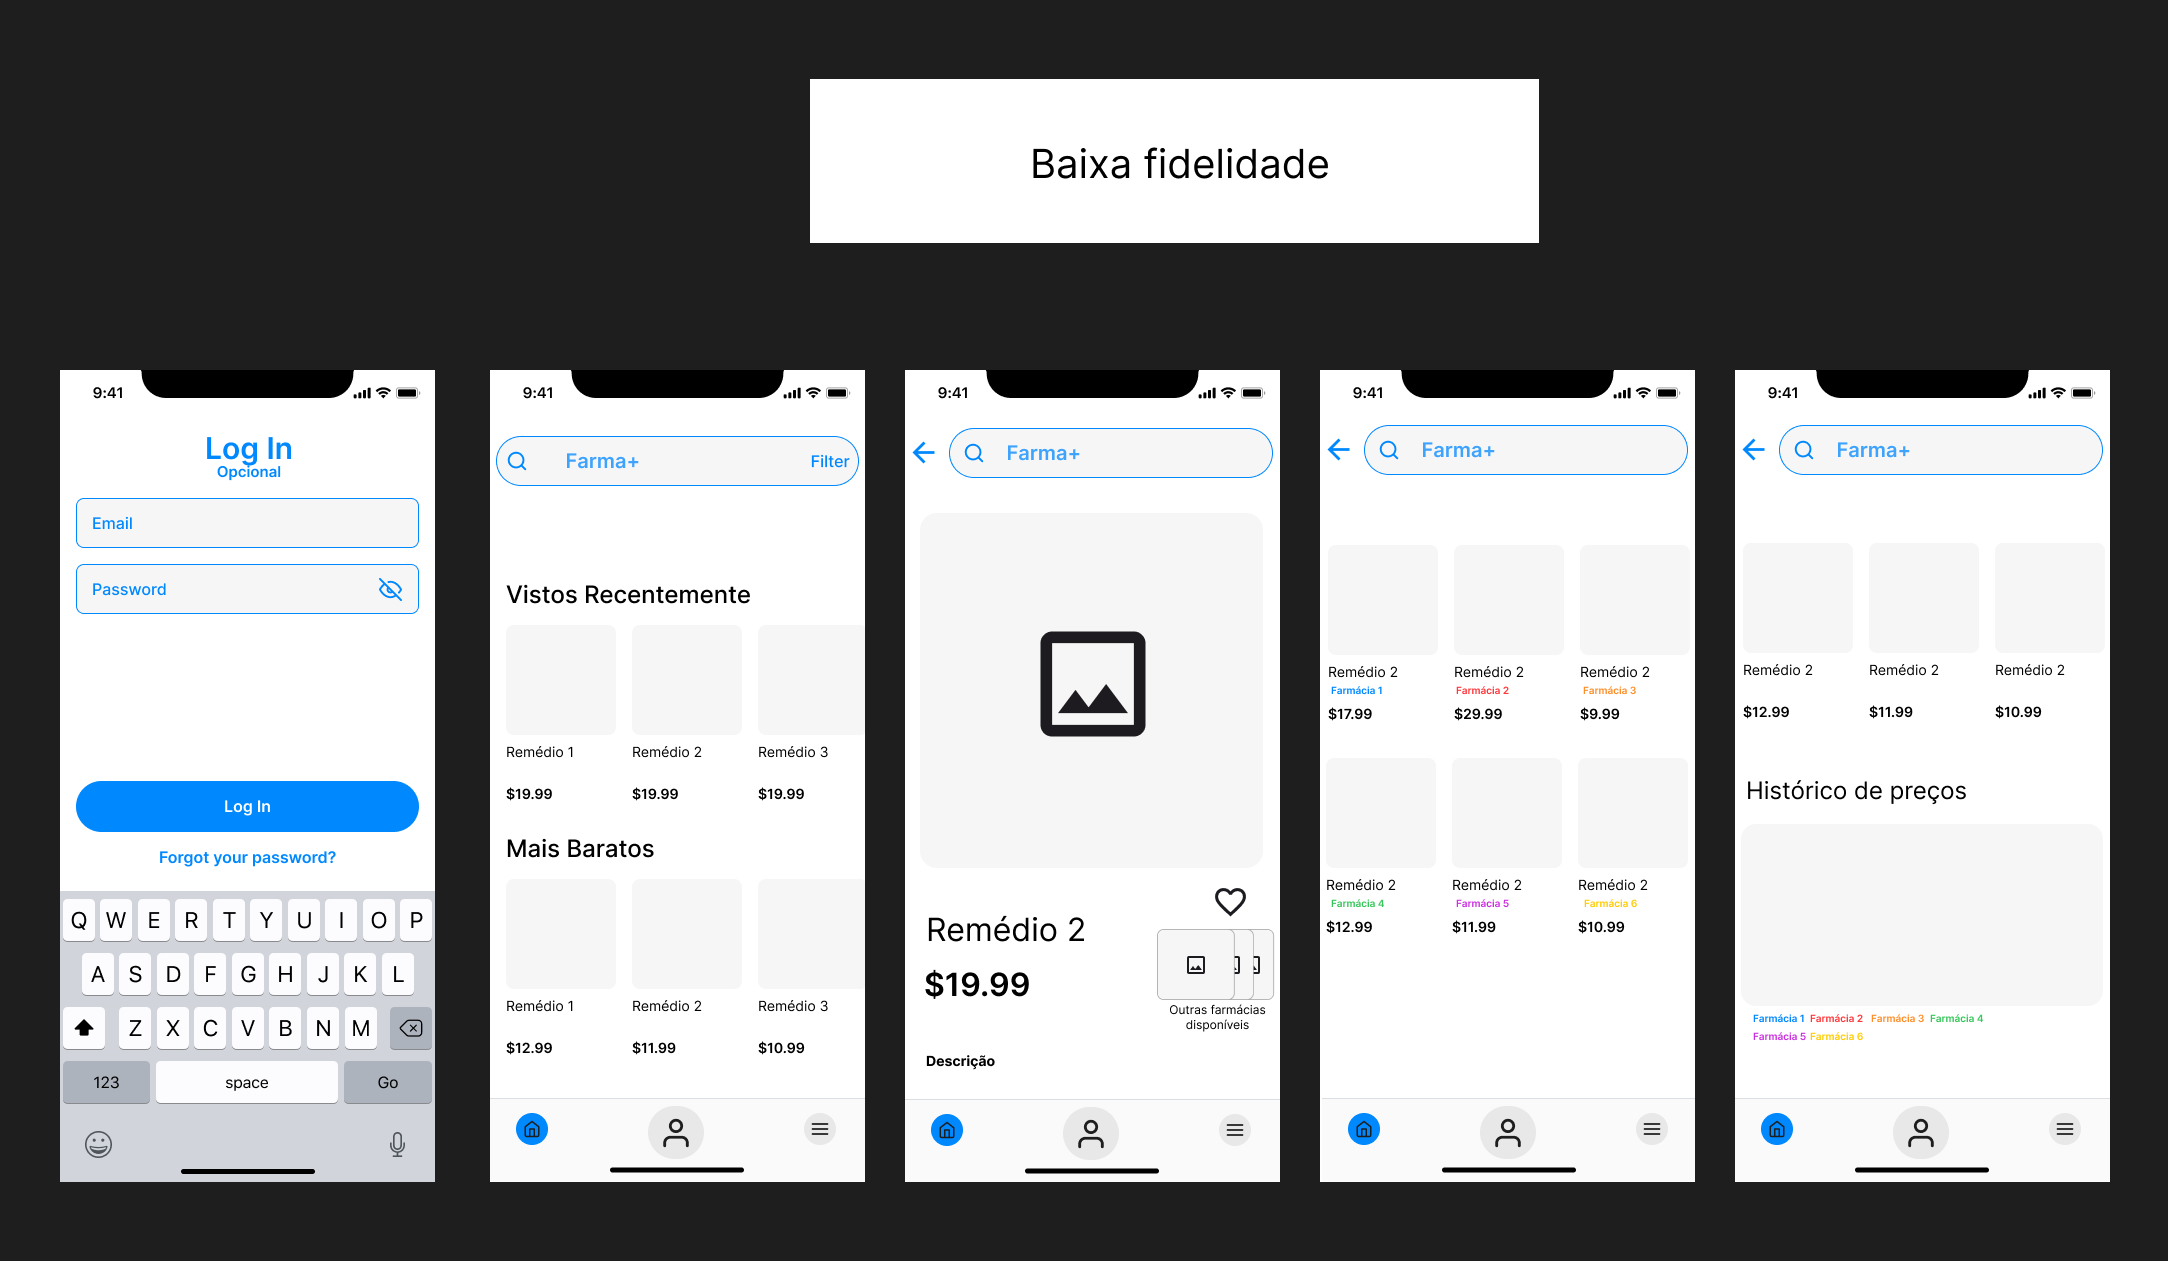
\includegraphics[width=\textwidth]{figures/prototipo-telas.png} 
    \fonte{Elaborado pelos autores (2026).}
\end{figure}

A navegação ilustrada reflete os seguintes módulos funcionais da aplicação, com ênfase nas diretrizes de acessibilidade aplicadas:

\begin{itemize}
    \item \textbf{Tela Inicial (Home):} Representada na primeira visualização, atua como o ponto de entrada do usuário. Destaca a barra de pesquisa global no topo, convidando a ação principal do sistema. Abaixo, apresenta categorias rápidas de navegação visual (como Genéricos, Higiene e Dermocosméticos) e um carrossel horizontal sugerindo as farmácias integradas à plataforma. Sob a ótica da acessibilidade, a barra de pesquisa apresenta alto contraste em relação ao fundo, facilitando a identificação imediata. Os ícones das categorias possuem traços espessos e semântica clara, auxiliando usuários com baixa visão ou barreiras cognitivas na compreensão imediata da navegação não textual.
    
    \item \textbf{Fluxo de Login e Autenticação:} A segunda tela detalha a interface de acesso, essencial para desbloquear recursos atrelados ao perfil, como o monitoramento de preços (RF03). O design minimalista foca nos campos de credenciais (e-mail e senha) e oferece a recuperação de acesso ou o redirecionamento para o cadastro de novos usuários. Do ponto de vista da acessibilidade motora e visual, os campos de formulário (\textit{inputs}) possuem dimensionamento adequado de altura para atuar como alvos de toque (\textit{touch targets}) confortáveis. Adicionalmente, o botão de ação principal utiliza cores com elevado índice de contraste (em conformidade com as diretrizes WCAG), assegurando a legibilidade e a usabilidade para usuários com diferentes graus de daltonismo.
    
    \item \textbf{Resultados de Pesquisa e Comparação:} A terceira tela ilustra o núcleo funcional do aplicativo. Ao buscar por um produto, o sistema renderiza os cartões de exibição (RF05). Cada cartão consolida a foto do medicamento, o laboratório responsável e o valor da oferta. Destaca-se a integração com o motor de geolocalização (RF06), exibindo a quilometragem exata entre o usuário e a farmácia que detém aquele estoque. Em termos de design inclusivo, os cartões empregam uma rígida hierarquia visual. O uso de pesos tipográficos distintos (negrito para a variável de maior interesse, o preço) e o espaçamento em branco (\textit{whitespace}) adequado previnem o sobrecarregamento cognitivo, facilitando a leitura rápida e a distinção visual entre os dados farmacológicos e a distância métrica.
    
    \item \textbf{Barra de Navegação Inferior (\textit{Bottom Navigation}):} Presente em toda a jornada principal, a barra garante acesso imediato às rotas de Início, Busca, Favoritos (itens salvos para monitoramento) e Perfil, assegurando uma transição fluida entre os diferentes contextos de uso do aplicativo. Para atender aos padrões de acessibilidade, os ícones da barra de navegação são obrigatoriamente acompanhados de rótulos textuais de apoio, eliminando ambiguidades interpretativas. O contraste dinâmico entre o estado ativo e inativo dos itens fornece um \textit{feedback} visual contínuo, orientando o usuário sobre sua exata localização na arquitetura da informação.
\end{itemize}

\section{Plano de Testes} %

Este tópico apresenta o plano de testes da plataforma Preço Bão, mantendo alinhamento com a especificação de requisitos, modelagem, arquitetura e protótipo de interface documentados no projeto. O objetivo é planejar a verificação e validação das funcionalidades principais do sistema, incluindo pesquisa de medicamentos, comparação de preços, geolocalização, autenticação, favoritos, monitoramento de preços e rotina automatizada de coleta de dados por \textit{web scraping}.

\subsection{Introdução} %

\begin{itemize}
    \item \textbf{Nome do sistema:} Plataforma Preço Bão.
    \item \textbf{Objetivo do software:} Permitir que consumidores pesquisem, comparem e monitorem preços de medicamentos e produtos de farmácia por meio de aplicativo móvel e versão web.
    \item \textbf{Problema que o sistema busca resolver:} A dificuldade do consumidor em comparar preços de medicamentos em diferentes farmácias, considerando volatilidade dos valores, disponibilidade estimada em estoque e distância até os estabelecimentos.
    \item \textbf{Público-alvo:} Consumidores finais que compram medicamentos de uso contínuo, produtos de farmácia, higiene e dermocosméticos, especialmente usuários que desejam economizar tempo e dinheiro.
    \item \textbf{Integrantes do grupo:} Aurora Drumond Costa Magalhães, Ana Clara de Souza e Kayke Wellington.
\end{itemize}

\subsection{Escopo dos Testes} %

O escopo dos testes contempla as funcionalidades centrais necessárias para validar o funcionamento do sistema sob a perspectiva do usuário final, do banco de dados e dos serviços de retaguarda.

\textbf{Funcionalidades que serão testadas:}
\begin{itemize}
    \item Cadastro, \textit{login}, autenticação e recuperação de senha de usuários.
    \item Pesquisa de medicamentos e produtos de farmácia.
    \item Exibição dos resultados em cartões padronizados, contendo laboratório, preço, farmácia, disponibilidade estimada e origem da oferta.
    \item Ordenação neutra dos resultados por menor preço ou menor distância.
    \item Cálculo de distância geográfica mediante autorização de localização.
    \item Favoritar medicamentos e produtos para acompanhamento posterior.
    \item Exibição de histórico ou gráfico de variação de preços.
    \item Rotina automatizada de \textit{web scraping}, tratamento de falhas e persistência dos dados coletados.
    \item Integração entre \textit{frontend} React Native, \textit{backend} FastAPI e banco PostgreSQL.
\end{itemize}

\textbf{Funcionalidades fora do escopo:}
\begin{itemize}
    \item Compra, pagamento ou reserva de medicamentos dentro da plataforma.
    \item Confirmação oficial de estoque em tempo real diretamente no sistema da farmácia.
    \item Entrega em domicílio ou integração com sistemas logísticos.
    \item Validação regulatória completa de prescrição médica ou controle de receita.
\end{itemize}

\textbf{Limitações identificadas:}
\begin{itemize}
    \item A disponibilidade em estoque é uma estimativa e deve ser confirmada no local pelo usuário.
    \item A precisão dos dados depende da qualidade das páginas públicas das farmácias e da rotina de extração.
    \item A geolocalização depende da permissão do usuário e da precisão do dispositivo.
    \item Testes de carga em ambiente acadêmico podem não representar a escala real de produção.
\end{itemize}

\subsection{Requisitos a Serem Testados} %

Os requisitos selecionados foram extraídos da especificação do projeto e representam os comportamentos funcionais e critérios de qualidade mais relevantes para a validação da plataforma.

\begin{quadro}[H]
    \centering
    \caption{Requisitos funcionais selecionados para teste}
    \label{qua:testes_rf}
    \begin{tabularx}{\textwidth}{|c|X|}
        \hline
        \textbf{ID} & \textbf{Requisito a ser testado} \\
        \hline
        RF01 & \textbf{Extração Resiliente de Dados:} validar se a rotina de \textit{web scraping} coleta dados de farmácias, registra falhas em \textit{log} e continua a varredura nas demais fontes. \\
        \hline
        RF03 & \textbf{Gestão de Usuários:} verificar cadastro, autenticação, \textit{login} e recuperação de senha do usuário. \\
        \hline
        RF04 & \textbf{Pesquisa e Neutralidade Algorítmica:} validar busca por medicamentos e ordenação por menor preço ou menor distância. \\
        \hline
        RF05 & \textbf{Exibição em Cartões:} verificar se os resultados são exibidos com informações de laboratório, preço e melhores ofertas. \\
        \hline
        RF06 & \textbf{Cálculo de Distância Geográfica:} verificar cálculo de distância até as farmácias após permissão de localização. \\
        \hline
        RF07 & \textbf{Salvamento de Produtos:} validar a opção de favoritar medicamentos de uso contínuo na conta do usuário. \\
        \hline
        RF08 & \textbf{Monitoramento de Preços:} verificar o histórico ou gráfico de flutuação de preços dos itens salvos. \\
        \hline
    \end{tabularx}
    \fonte{Elaborado pelos autores (2026).}
\end{quadro}

\begin{quadro}[H]
    \centering
    \caption{Requisitos não funcionais selecionados para teste}
    \label{qua:testes_rnf}
    \begin{tabularx}{\textwidth}{|c|X|}
        \hline
        \textbf{ID} & \textbf{Requisito a ser testado} \\
        \hline
        RNF01 & \textbf{Performance da API:} validar resposta de requisições de pesquisa em até 500 milissegundos no percentil 95. \\
        \hline
        RNF02 & \textbf{Arquitetura do Frontend:} verificar execução do aplicativo React Native/Expo com TypeScript para Android e iOS. \\
        \hline
        RNF04 & \textbf{Segurança e Criptografia:} validar armazenamento de senhas com \textit{hash} forte e comunicação protegida por HTTPS/TLS. \\
        \hline
        RNF05 & \textbf{Privacidade (LGPD):} verificar se coordenadas geográficas são processadas em memória e descartadas após uso. \\
        \hline
        RNF08 & \textbf{Orquestração Local:} validar provisionamento do ambiente com \file{docker-compose.yml}. \\
        \hline
        RNF10 & \textbf{CI/CD e Qualidade:} verificar bloqueio de \textit{Pull Requests} que falhem em testes ou análise estática. \\
        \hline
    \end{tabularx}
    \fonte{Elaborado pelos autores (2026).}
\end{quadro}

\subsection{Estratégia de Testes} %

A estratégia de testes combina validação funcional, integração, persistência, segurança, interface e desempenho, cobrindo tanto o fluxo do usuário quanto os componentes internos da arquitetura.

\begin{quadro}[H]
    \centering
    \caption{Estratégias de teste propostas}
    \label{qua:estrategias_teste}
    \begin{tabularx}{\textwidth}{|l|X|X|X|}
        \hline
        \textbf{Tipo de Teste} & \textbf{Objetivo} & \textbf{Técnica Utilizada} & \textbf{Resultado Esperado} \\
        \hline
        Teste Funcional & Verificar se as funcionalidades do sistema executam corretamente conforme os requisitos. & Executar fluxos com dados válidos e inválidos em cadastro, \textit{login}, pesquisa, favoritos e histórico. & O sistema deve responder corretamente às ações do usuário e exibir mensagens adequadas. \\
        \hline
        Teste de Interface & Avaliar usabilidade, organização visual e navegação entre as telas. & Navegar pelo aplicativo validando botões, campos, cartões, barra inferior, contraste e rótulos. & As telas devem ser intuitivas, legíveis e permitir navegação sem ambiguidade. \\
        \hline
        Teste de Banco de Dados & Verificar persistência, consulta e integridade das informações. & Inserir, consultar e validar registros em Usuario, CatalogoBase, Farmacia, OfertaFarmacia, Favorito e HistoricoPreco. & Os dados devem ser armazenados e recuperados sem inconsistências. \\
        \hline
        Teste de Segurança & Garantir proteção de credenciais e acesso restrito a recursos autenticados. & Testar \textit{login} inválido, acesso a favoritos sem autenticação, \textit{hash} de senha e descarte de localização. & Usuários não autorizados não devem acessar recursos restritos, e dados sensíveis não devem ser expostos. \\
        \hline
        Teste de Integração & Verificar comunicação entre \textit{frontend}, API, banco e rotina de \textit{scraping}. & Executar fluxo completo: coleta de dados, gravação no PostgreSQL, consulta via FastAPI e exibição no app. & Os módulos devem trocar informações corretamente e tratar falhas sem interromper o sistema. \\
        \hline
        Teste de Desempenho & Avaliar comportamento da API em pesquisas simultâneas. & Simular múltiplas requisições e medir tempo de resposta das buscas principais. & A API deve manter tempo de resposta compatível com RNF01. \\
        \hline
    \end{tabularx}
    \fonte{Elaborado pelos autores (2026).}
\end{quadro}

\subsection{Casos de Teste} %

Os casos de teste foram definidos para cobrir os fluxos principais da plataforma, priorizando funcionalidades críticas para a experiência do usuário e para a confiabilidade dos dados.

\begin{quadro}[H]
    \centering
    \caption{Casos de teste da plataforma Preço Bão - Prioridade Alta}
    \label{qua:casos_teste_alta}
    \small
    \begin{tabularx}{\textwidth}{|c|X|X|X|c|c|}
        \hline
        \textbf{ID} & \textbf{Caso de Teste} & \textbf{Entrada de Dados} & \textbf{Resultado Esperado} & \textbf{Prioridade} & \textbf{Status} \\
        \hline
        CT01 & Cadastro de usuário com dados válidos & Nome, e-mail válido e senha válida & Usuário cadastrado com sucesso e perfil criado. & Alta & Pendente \\
        \hline
        CT02 & Login com credenciais válidas & E-mail e senha corretos & Acesso permitido à conta do usuário. & Alta & Pendente \\
        \hline
        CT03 & Login com senha inválida & E-mail válido e senha incorreta & Sistema deve negar acesso e exibir mensagem de credenciais inválidas. & Alta & Pendente \\
        \hline
        CT04 & Pesquisa de medicamento existente & Nome de medicamento presente no catálogo & Sistema deve listar ofertas disponíveis em cartões padronizados. & Alta & Pendente \\
        \hline
        CT06 & Ordenação por menor preço & Busca com múltiplas ofertas & Resultados devem ser ordenados pelo menor preço, sem favorecimento de farmácia. & Alta & Pendente \\
        \hline
        CT07 & Ordenação por menor distância & Busca com permissão de localização ativa & Resultados devem ser ordenados pela menor distância calculada até as farmácias. & Alta & Pendente \\
        \hline
        CT09 & Favoritar medicamento autenticado & Usuário logado seleciona favorito & Produto deve ser associado ao usuário e aparecer na tela de favoritos. & Alta & Pendente \\
        \hline
        CT10 & Favoritar medicamento sem login & Usuário não autenticado tenta favoritar & Sistema deve solicitar login antes de salvar o produto. & Alta & Pendente \\
        \hline
        CT12 & Scraping com falha parcial & Uma fonte indisponível durante a coleta & Erro deve ser registrado em log e a varredura deve continuar nas demais farmácias. & Alta & Pendente \\
        \hline
        CT13 & Persistência de oferta coletada & Produto, farmácia, preço e disponibilidade coletados & Dados devem ser gravados em OfertaFarmacia e vinculados ao catálogo e à farmácia. & Alta & Pendente \\
        \hline
    \end{tabularx}
    \fonte{Elaborado pelos autores (2026).}
\end{quadro}

\begin{quadro}[H]
    \centering
    \caption{Casos de teste da plataforma Preço Bão - Prioridade Média}
    \label{qua:casos_teste_media}
    \small
    \begin{tabularx}{\textwidth}{|c|X|X|X|c|c|}
        \hline
        \textbf{ID} & \textbf{Caso de Teste} & \textbf{Entrada de Dados} & \textbf{Resultado Esperado} & \textbf{Prioridade} & \textbf{Status} \\
        \hline
        CT05 & Pesquisa sem resultado & Nome inexistente ou inválido & Sistema deve informar que nenhum produto foi encontrado. & Média & Pendente \\
        \hline
        CT08 & Negar permissão de localização & Usuário recusa acesso à localização & Sistema deve manter pesquisa por preço e informar indisponibilidade da ordenação por distância. & Média & Pendente \\
        \hline
        CT11 & Exibir histórico de preços & Produto salvo com registros em HistoricoPreco & Sistema deve apresentar gráfico ou lista de variação de preços das últimas semanas. & Média & Pendente \\
        \hline
    \end{tabularx}
    \fonte{Elaborado pelos autores (2026).}
\end{quadro}

\begin{quadro}[H]
    \centering
    \caption{Casos de teste da plataforma Preço Bão - Prioridade Baixa}
    \label{qua:casos_teste_baixa}
    \small
    \begin{tabularx}{\textwidth}{|c|X|X|X|c|c|}
        \hline
        \textbf{ID} & \textbf{Caso de Teste} & \textbf{Entrada de Dados} & \textbf{Resultado Esperado} & \textbf{Prioridade} & \textbf{Status} \\
        \hline
        CT14 & Teste de desempenho da busca & Múltiplas requisições simultâneas de pesquisa & API deve responder dentro do limite esperado para o cenário de teste. & Baixa & Pendente \\
        \hline
    \end{tabularx}
    \fonte{Elaborado pelos autores (2026).}
\end{quadro}

\subsection{Infraestrutura e Recursos de Teste} %

\begin{itemize}
    \item \textbf{Sistema operacional:} Windows 10/11 ou Linux para execução dos serviços de desenvolvimento e testes.
    \item \textbf{Banco de dados:} PostgreSQL, conforme especificação de persistência do projeto.
    \item \textbf{Backend:} Python com FastAPI, SQLAlchemy ORM, Pydantic e execução assíncrona.
    \item \textbf{Frontend:} React Native com Expo e TypeScript.
    \item \textbf{Navegador:} Google Chrome, Microsoft Edge ou navegador compatível para validação da versão web e consumo da API.
    \item \textbf{Ferramentas:} Visual Studio Code, Docker, docker-compose, Git/GitHub, GitHub Actions, ESLint, Ruff e ferramentas de teste da API.
    \item \textbf{Equipamentos:} Computador de desenvolvimento e smartphone ou emulador Android/iOS para validação do aplicativo móvel.
\end{itemize}

\subsection{Equipe e Responsabilidades} %

As responsabilidades foram distribuídas conforme os papéis necessários para planejamento, execução, registro e revisão das atividades de teste.

\begin{quadro}[H]
    \centering
    \caption{Equipe e responsabilidades}
    \label{qua:equipe_responsabilidades}
    \begin{tabularx}{\textwidth}{|l|X|}
        \hline
        \textbf{Integrante} & \textbf{Função} \\
        \hline
        Aurora Drumond Costa Magalhães & Elaboração dos casos de teste e validação dos requisitos funcionais. \\
        \hline
        Ana Clara de Souza & Execução dos testes de interface, autenticação, favoritos e registro das falhas encontradas. \\
        \hline
        Kayke Wellington & Execução dos testes de \textit{backend}, banco de dados, \textit{scraping}, desempenho e integração. \\
        \hline
        Grupo & Revisão final do plano de testes, consolidação dos resultados e validação do documento. \\
        \hline
    \end{tabularx}
    \fonte{Elaborado pelos autores (2026).}
\end{quadro}

\subsection{Cronograma de Testes} %

O cronograma a seguir organiza as principais etapas previstas para a realização dos testes da plataforma.

\begin{quadro}[H]
    \centering
    \caption{Cronograma simplificado de testes}
    \label{qua:cronograma_testes}
    \begin{tabularx}{\textwidth}{|X|l|c|}
        \hline
        \textbf{Atividade} & \textbf{Responsável} & \textbf{Prazo} \\
        \hline
        Planejamento dos testes & Grupo & 03/06/2026 \\
        \hline
        Elaboração dos casos de teste & Aurora Drumond Costa Magalhães & 08/06/2026 \\
        \hline
        Preparação do ambiente de teste & Kayke Wellington & 12/06/2026 \\
        \hline
        Execução dos testes funcionais e de interface & Ana Clara de Souza & 16/06/2026 \\
        \hline
        Execução dos testes de banco, integração, segurança e desempenho & Kayke Wellington & 13/06/2026 \\
        \hline
        Registro de falhas e análise dos riscos & Grupo & 14/06/2026 \\
        \hline
        Correção, validação e revisão final & Grupo & 17/06/2026 \\
        \hline
    \end{tabularx}
    \fonte{Elaborado pelos autores (2026).}
\end{quadro}

\subsection{Registro de Defeitos e Riscos} %

O registro de defeitos e riscos antecipa problemas que podem ocorrer durante a execução dos testes e durante a evolução do projeto.

\begin{quadro}[H]
    \centering
    \caption{Possíveis defeitos identificados}
    \label{qua:defeitos_identificados}
    \begin{tabularx}{\textwidth}{|c|X|X|X|}
        \hline
        \textbf{ID} & \textbf{Falha identificada} & \textbf{Possível Causa} & \textbf{Solução Proposta} \\
        \hline
        RFAL01 & Login não permite acesso mesmo com credenciais corretas. & Erro na validação da senha, \textit{hash} incorreto ou falha de comunicação com o banco. & Revisar autenticação, geração de \textit{hash} e consulta do usuário no \textit{backend}. \\
        \hline
        RFAL02 & Pesquisa retorna produtos duplicados ou sem preço. & Falha no tratamento dos dados coletados pelo \textit{scraping} ou inconsistência em OfertaFarmacia. & Revisar normalização do catálogo, chaves de relacionamento e filtros da consulta. \\
        \hline
        RFAL03 & Distância geográfica exibida incorretamente. & Erro no cálculo de latitude/longitude, permissão negada ou coordenadas inválidas. & Validar fórmula de cálculo, tratar ausência de localização e testar valores conhecidos. \\
        \hline
        RFAL04 & Histórico de preços não aparece para produto favoritado. & Ausência de registros em HistoricoPreco ou erro de vínculo com usuário/produto. & Revisar rotina de gravação histórica e relacionamento entre Favorito e CatalogoBase. \\
        \hline
    \end{tabularx}
    \fonte{Elaborado pelos autores (2026).}
\end{quadro}

\begin{quadro}[H]
    \centering
    \caption{Riscos relacionados ao projeto e aos testes}
    \label{qua:riscos_projeto}
    \begin{tabularx}{\textwidth}{|c|X|X|X|}
        \hline
        \textbf{ID} & \textbf{Risco identificado} & \textbf{Impacto} & \textbf{Mitigação} \\
        \hline
        R01 & Mudança no layout ou na estrutura dos sites das farmácias. & Pode interromper ou reduzir a qualidade da extração de dados por \textit{scraping}. & Criar \textit{logs} detalhados, testes automatizados para os \textit{scrapers} e estratégia de adaptação por farmácia. \\
        \hline
        R02 & Ambiente de testes diferente do ambiente real de produção. & Resultados de desempenho e integração podem não representar a operação real. & Documentar limitações, executar testes em ambiente controlado e repetir cenários críticos em infraestrutura próxima da final. \\
        \hline
        R03 & Exposição indevida de dados pessoais ou localização. & Pode causar não conformidade com a LGPD e perda de confiança do usuário. & Validar descarte das coordenadas, revisar permissões e testar fluxos de privacidade. \\
        \hline
    \end{tabularx}
    \fonte{Elaborado pelos autores (2026).}
\end{quadro}
% \chapter{Conclusão}

% ----------------------------------------------------------
% ELEMENTOS PÓS-TEXTUAIS
% ----------------------------------------------------------
\postextual

% CONFIGURAÇÃO CORRETA DA BIBLIOGRAFIA
\bibliographystyle{abntex2-alf} % Define o estilo ABNT (Autor-Data)
\bibliography{references}      % Chama o arquivo .bib



\end{document}